%%\documentclass{umassthesis}          % for Ph.D. dissertation or proposal
\documentclass[thesis,proposal]{umassthesis}  % for Master's thesis

%
\usepackage{url}
\usepackage{amsmath}
\usepackage{pdfpages}
\usepackage{graphicx}

%%
%% If you have enough figures or tables that you run out of space for their
%% numbers in the List of Tables or List of figures, you can use the following
%% command to adjust the space left for numbers.  The default is shown:
%%
%% \setlength{\tablenumberwidth}{2.3em}

%% Use the hyperref package if you're producing a version for online
%% distribution and you want hyperlinks.  Note that the Grad School doesn't want
%% their PDF viewers to colorize or otherwise highlight the links; use the
%% hidelinks option to hyperref to avoid decorating links.
%\usepackage[hidelinks]{hyperref}

%% One way of formatting the epigraph/frontispiece is to use this package.
%\usepackage{epigraph}

\begin{document}

%%
%% You must fill in all of these appropriately
\title{BrightSpot:\protect\\Optimizing the Cost of Executing Batch-Interactive Workloads in the Cloud
  \protect\\}
\author{Justin Mills}
\date{September 2016} % The date you'll actually graduate -- must be
                     % February, May, or September
\copyrightyear{2016}
\bachelors{B.Sc.}{University of Massachusetts, Amherst}
\masters{M.Sc.}{University of Massachusetts, Amherst}

% \committeechair{B. B. Bahh}
\committeechair{David Irwin}
\firstreader{Tillman Wolf}
\secondreader{Michael Zink}
%\fifthreader{}            % Optional
%\sixthreader{}            % Optional
\departmentchair[Department Head]{Christopher V. Hollot} % Uses "Department Chair" as the title. To
% use an alternate title, such as "Chair", use \departmentchair[Chair]{Pete Shearer}
\departmentname{Electrical and Computer Engineering}


\degree{Master of Science in Electrical and Computer Engineering}{M.S.E.C.E.}


%%
%% These lines produce the title, copyright, and signature pages.
%% They are Mandatory; except that you could leave out the copyright page
%% if you were preparing an M.S. thesis instead of a PhD dissertation.
\frontmatter
\maketitle
\copyrightpage     %% not required for an M.S. thesis
\signaturepage

%%
%% Dedication is optional -- but this is how you create it
%\begin{dedication}              % Dedication page
%  \begin{center}
%    \emph{To those little lost sheep.} %Might want to change this
%  \end{center}
%\end{dedication}

%%
%% Acknowledgements are optional...yeah, right.
\chapter{Acknowledgments}             % Acknowledgements page
  I would like to thank all those who have given me their time and support in completing this proposal. Foremost of all I would like to thank Professor David Irwin for being my advisor. He has given me valuable guidance, has helped me design my thesis at every stage, and helped me to find my path whenever I've begun to get stuck.\par
  Next I would like to thank Xue Ouyang for sharing her knowledge and experiences from working with the spot market and AWS. 

%%
%%Abstract is MANDATORY. -- Except for MS theses
\begin{abstract}                % Abstract
  The use of cloud computing to make setting up and maintaining services easier
  is becoming more common every day. One major benefit is that it relieves the
  user of the need to buy new hardware to begin hosting a service that may require
  much computing power. The challenge that cloud users now face is how to
  minimize their costs while using cloud computing as a low-cost operational method.
  To accomplish this, I propose to develop BrightSpot, a system which makes use of the cloud market's
  cheap but unreliable services while maintaining a high level of availability for the
  minimum cost. 
  The key factor in BrightSpot's algorithm is analyzing the Amazon's spot market. Spot instances are a cost saving measure by Amazon that utilize the underutilized space on its active cloud servers to provide cloud users access to these servers, but can take the servers away at any time. BrightSpot analyzes the sale history to choose which spot instances will provide the lowest cost while also providing the highest amount of time available for use. With the best servers chosen, BrightSpot will then be able to maintain a reliable web service on these unreliable servers by calculating an amount of excess servers to maintain to provide backups to any servers that may fail. While holding these backup instances, BrightSpot will also be able to utilize this extra server space to perform some background, batch processing task, which does not require a guaranteed reliability, and thus increase the amount of work that can be done for an already reduced overhead cost.
\end{abstract}

%%
%% Preface goes here...would be just like Acknowledgements -- optional
%% \chapter{Preface} 
%% ...


%%
%% Table of contents is mandatory, lists of tables and figures are 
%% mandatory if you have any tables or figures; must be in this order.
\tableofcontents                % Table of contents
\listoftables                   % List of Tables
\listoffigures                  % List of Figures

%%
%% We don't handle List of Abbreviations
%% We don't handle Glossary

%%%%%%%%%%%%%%%%%%%%%%%%%%%%%%%%%%%%%%%%%%%%%%%%%%%%%%%%%%%%%%%%%%%%%%%%%
%% Time for the body of the dissertation
\mainmatter   %% <-- This line is mandatory

%%
%% If you want an introduction, which is not a numbered chapter, insert
%% the following two lines.  This is OPTIONAL:
\unnumberedchapter{Introduction}
Starting a web-based company is a very risky endeavor. Recent statistics place the start-up failure rate above 90\% for varying reasons \cite{startupReport}. This figure serves as an incredible deterrent for any who wish to start their own business. This risk exists with any new venture, be it a business idea or a simple life decision, but there are certainly more risks associated with failing at creating a business than with most such decisions. For instance, consider the start-up costs of a web-based companies. One of the largest costs in creating such a business is obtaining hardware that can support whatever product one hopes to create. This hardware must be obtained before any implementation can even be obtained, and should the company fall short for any reason, it represents a huge loss to any who invested in this company. This, however, is a concern that the cloud market has been designed to rectify.\par

The Cloud is a collection of hardware resources which are privately owned some companies and rented out for use by other companies. The cloud market takes many forms, such Google’s Compute Engine (GCE) and Amazon Web Service's Elastic Compute Cloud (AWS EC2), but each are fundamentally the same: users who wish to use these resources pay for the resources they want and are charged for the amount of time they use said resources. When the user selects the resources they wish to use, they agree to pay a set price for them and are guaranteed use of them for as long as they wish. This is the standard type of agreement and it is known as an On-Demand server agreement. However, like with any business model, there are certain inefficiencies which arise with this market. One such issue is that the owners of cloud resources have no control over which resources are requested and at what times certain instance types are desired. This creates some cases where cloud server owners have active servers that are not fully utilized.\par

The reason under-utilized servers present a problem for cloud providers is how much power is used by servers that are on but inactive. one can consider the case where only one user requests the highest speed server type from Google, but the user only wish to utilize 10\% of the host server's capacity. Google must now activate this server, and while it is only at 10\% utilization, its power consumption is very high comparatively, most likely around 50\% \cite{serverPowerUsage}. This leads to a situation where Google is paying more to sell this resource than they should have to, which is also a situation where providing access of this server to more users would cost nearly nothing. Seeing this issue, Amazon came up with a solution they called EC2 Spot Instances \cite{awsSpotInfo}. Spot Instances are Cloud computing resources that make up the underutilized space on currently active Amazon servers. Spot Instances are auctioned off to the highest bidder at a cost that is always below the On-Demand price of the resource. The catch to these instances is that they are not guaranteed as available to any user for any amount of time and thus can be taken away as soon as someone is willing to pay more for the resource or when the server no longer has room for that spot instance.\par

These spot instances, and their equivalents at other companies such as Google, have provided a unique opportunity. Companies seeking to minimize costs have the option to “take a chance” on these unreliable resources and utilize them as opposed to on-demand servers at full price. Initially, this would seem a heavy risky, especially for new companies who can’t risk intermittent service outages while trying to establish themselves. However, there would appear to be ways to avoid losing service while still benefiting from these affordable prices. The problem now is how can one implement a service with some given availability for the minimum cost available and whether it is possible to do so by utilizing spot instances.\par

To solve this problem, we propose to create BrightSpot, a system designed to manage web applications with some desired availability utilizing Amazon EC2 Spot Instances to provide the lowest operating costs possible. A user wishing to utilize BrightSpot will provide it with a desired system availability as well as an initial amount of computing resources desired. BrightSpot will then use the historical Amazon Spot Market price data to determine the best spot choices to make the cheapest system possible. It will accomplish this by looking at three key factors for each spot instance type in the pricing history: cost per computing resources relevant to the user's needs, availability of that spot instance at the optimal price, and correlation with other spot instance types that may be obtained. These three factors will then be associated with each other to find the best price per availability percentage that each instance can provide. With this information, we will be able to predict which spot instance purchasing decisions will most likely provide the best overall cost for implementing the desired web service.\par

There is also a secondary benefit to be seen in utilizing spot instances in this way. In order to maintain high availability with low availability server instances, the solution will require obtaining more computing resources at any given time, providing thus far unused resources. It is now possible to utilize these resources for no extra cost to accomplish some task that has no necessary availability and can be worked on and completed at any rate that the servers happen to be available. Our hypothesis is that by utilizing the pricing history of the spot market to make the best purchasing decisions, it is possible to create a reliable web service for less cost than using fully reliable cloud instances. In evaluating our hypothesis, we will make the following contributions:\par

{\bf Best Cost Prediction:} Assessing the best cost scenario will be the first step in choosing which spot instances to choose. By using the history data provided by Amazon, we will be able to predict the prices we can expect to pay for any given instance type across its lifespan as well as what amount of availability it will provide for that cost. Further, we can assess the correlation of servers to see how much our system availability will increase by adding a given server type so that we are able to make the best decisions for the entire life of the system.

{\bf Maintaining Desired Availability:} We will utilize the best cost predictions to determine which instances top obtain to support our system. This will give us a predicted availability of whatever percentage of whatever the user chooses. However, the volatility of the spot market will still cause the loss of instances and the need to exchange some instances for others. To address this, Kubernetes will be used as the primary method of managing cloud resources and ensuring we have the desired number of instances.

{\bf Implementation and Evaluation:} Once this analysis and preparation is done, we propose to implement the system to evaluate our hypothesis. The system will be implemented using Java and deployed on Amazon EC2. We will compare the cost experienced by the implementation to that predicted by the cost analyzer. We will also assess how frequently making our purchasing decisions based on history data provided better results than if we had taken into account current spot prices as well. Next, we will determine if we achieved our goal of maintaining the desired amount of availability for the system by determining the amount of down time experienced. Finally, the amount of excess resources obtained will be tabulated in such a way so as to determine the capabilities a user might be able to have by making use of it.










\chapter{Background and Motivation}

In this chapter, we will explain many of the terms and services we will be utilizing to create our system design. We will also give a more in depth explanation of the problems we believe our system will be able to solve and how it addresses each.

\section{The Cloud}

Resources in the cloud are requested by the size of the resource, its physical location, and the provider. 

\subsection{Choice of Cloud Provider}

The initial considerations for which cloud provider to use mainly consisted of deciding between Google and Amazon, as they each offered their own cheaper, unreliable instances to form a solution around. Amazon EC2 offers the spot market, where users bid on the temporary resources and the highest bidders obtain the instance. The instance is given to them at the current price regardless of their bids, but taken away from them when the price of the system exceeds their bid. GCE, on the other hand, offers Preemptible Virtual Machines (VMs). These instances are similar in that they can be taken from the user at any time that they cease to be available, but they differ by removing the spot market bidding system. Instead, GCE users are simply charged approximately 40\% of their typical per hour costs for these unreliable instances \cite{googleComputePricing}. \par

This decision was given considerable attention, as each had very useful benefits as well as some drawbacks that would influence our ability to make the best purchasing choices. Without reliably being able to make smart purchasing decisions, the system would not be able to guarantee that it was providing the user with an optimal or near optimal solution.\par

Amazon has a much more established spot market, providing very useful past data about their various spot markets that can be used to accurately predict the most likely future prices and make the most informed purchasing decisions. However, the Amazon Spot Market is far more complex and utilizes a bidding system which adds to the difficulty in making an optimal algorithm. Google’s Preemptible VMs offer a fixed price and a much more fluid integration with Kubernetes, a service that will be utilized to manage server instances \cite{introToKubernetes}. They are also newer, however, and thus lack the history data of revocations that would be useful in making confident purchasing decisions. Additionally, GCE puts an absolute limit of 24 hours on any preemptible instance they sell, meaning that there must be a complete turnover of instances within a 24-hour period. While we will aim to minimize the overhead experienced in such a transition, limiting the number of transitions will also be pivotal in ensuring the lowest cost for the highest performance.\par

By using Kubernetes with EC2 rather than GCE, however, we will increase the complexity of our system as the two were not designed with one another in mind as GCE and Kubernetes were. Using GCE was the intention for Kubernetes very early on. In the end, the deciding factor was the fact that consistent, reliable purchasing decisions could not be made unless the decisions were not made solely on the best cost option currently, but on the availability of each instance at that cost as well. This meant that EC2 was necessary for our uses. Without the ability to analyze historical data, we would be making blind decisions and would ensure we encounter heavy instance turnover rates and may experience blackouts frequently.\par


\subsection{Amazon AWS}


There are numerous terms which must be defined to understand how Amazon AWS has been utilized and its history analyzed. A Region is a geographic area that every user is separated into. Every user has access to exactly one region and may only use resources from this Region \cite{ec2RegionsAndAZ}. Regions are all entirely separate and any communication between Regions is done via the internet.\par

Each Region is further divided in Availability Zones. An Availability Zone is also independent from other Availability Zones in the same Region in the sense that the server instances in each are independent \cite{ec2RegionsAndAZ}. This means that a t2.nano server request (the smallest type available from amazon) from availability zone a will be not affect any requests for the same server type in availability zone b. However, all availability zones within the same Region are interconnected so that an application making use of a server instance in zone a can send the traffic that was directed towards it to an instance in zone b should the instance in zone a fail.\par

Within each Availability Zone, a user is able to select the server instance type or types that they would like to purchase and use. The type of server instance that the user selects determines the hardware available on that server that is now able to be used by the user \cite{amazonEC2Pricing}. They are generally categorized by their processor speed, number of processor cores, and amount of Random Access Memory (RAM), however, some also have additional features such as excess storage space and high end graphics. The price predictably increases as instance resources increase, however different instance types are optimized in different ways. This means that some types utilize massive Ram while keeping a modest processor, and others will have a good balance between the two \cite{amazonEC2Pricing}.\par

The spot market history data provided by Amazon stretches back 60 days and is incredibly verbose. This includes data for every instance type, in each availability zone, in any given region with all associated costs presented and the times at which each purchase was made. This wealth of information is perfect for analyzing to make the best future purchasing decisions.\par




\section{Availability}

Once a desired availability is determined, BrightSpot will need a way of maintaining the instances we have obtained to hold this availability at all times. To maintain the correct number of servers, we have decided to use the container manager Kubernetes.

\subsection{Kubernetes}

Kubernetes is a system designed to manage and maintain containerized applications. Kubernetes creates containers, which are sealed application packages that exist as seemingly separated portions of a server resource. Essentially, these containers are treated as independent instances of computing resources, like separate VM instances, and are managed as such, but which are actually created by dividing a larger machine up so that you can make more efficient use out of this machine. While containers and Virtual Machines are very similar in their respective uses, there are distinct benefits to each. A Virtual Machine has the benefit of flexibility. By utilizing a Virtual Machine, one could choose to use any Operating System they wanted to use regardless of that of the host.\par

The benefit to using Containers, however, is that they utilize the Operating System of their host, thus negating the overhead and resource wasted by implementing a separate Operating System on top of another Operating System. By using Containers and minimizing or eliminating this waste of computer resources, we reduce the amount of computing resources we require and can save on operating costs. The only requirement to make use of Containers in the cloud is that you must be able to create your service in the type of environment provided by the cloud service providers, but as they offer very typical Operating System choices this is easily done.\par

Kubernetes then organizes these containers into pods, which are groups of containers that work together to achieve some goal. Pods are the smallest deployable units as viewed by Kubernetes \cite{openShiftGuidePods}. Each pod can contain from one to any number of containers, however all containers within a pod need to exist on the same physical or virtual host. Kubernetes creates pods based on need. It uses a replication controller and a desired state value to determine how many pods should exist at any time. If this desired state is not met, the number of active pods is either increased or decreased by creating or deactivating pods. Every pod has a template that it is created from, so in the case that Kubernetes must create more pods, like at system start-up or when traffic increases enough, it refers to the template of a pod that is needed and creates a pod from that template.\par

Kubernetes also has something known as a Service to manage Pods. There is an important abstraction between the service we are trying to create and what is meant when referring to a Kubernetes Service. Our service will be a simple web application of some type. A Kubernetes service is simply another component of the Kubernetes system. The Kubernetes service serves two crucial roles: to act as a staple, fixed component that is not as disposable as individual pods, and to provide load balancing for the pods we have available. A Kubernetes service exists on the master node, and thus it should never be in danger of failing as our master node should never be lost. Each service targets a specific type of pod with a specific label and a specific port. The service has an IP address given to it, referred to as the “cluster IP” \cite{googleGuideServices}. Requests for the desired functionality of the pods managed by a service are received by the service at this IP and then distributed to the pods in a round robin fashion to keep pods under equal load.\par

	Kubernetes uses a Master-Minion structure to manage resources, meaning we divide up our resources into a master node and minion nodes. In this case, a node refers to an amount of computing resources needed for something. There is only ever one Master node and it resides on a physical or virtual resource that should never be revocable. The Master node contains the main instance of Kubernetes as well as the top level of our management system which will interact with Kubernetes. The minions, however, can reside on revocable, lossy instances. For our purposes this will be the vast majority of them. It should be noted that there is nothing preventing the creation of one or more pods on the Master node’s instance as long as the necessary resources are available. The Master node manages all instances of minion nodes in numerous ways and decides which minions are to be kept, which are to be disposed of, and when more minions need to be activated.\par
    
Kubernetes utilizes a Replicated State Machine approach to providing web services. This means that Kubernetes creates a certain number of copies of a service and distributes user requests to access this service throughout the available pods. The number of copies of a service is called the desired state and is a setting within Kubernetes. When something happens to change the number of available services, such as one cloud instance failing or being revoked, Kubernetes will see some number of pods have failed and will obtain the necessary resources and create more until the desired state is met. To create an identical pod, Kubernetes references the label attached to the pod that has failed and accesses a template of that pod to create the next instance.\par

	The use of the desired state and template files to manage resources makes Kubernetes ideal for integration into a cloud based service utilizing unstable instances. It is a system designed entirely to deal with faults that happen and take resources away from a system. When utilizing lossy instances such as EC2 Spot Instances as we propose to do, a system with fault tolerance built in is not only beneficial, but essential.\par
    
\subsection{Maintaining Availability}

Faults can be caused by a number of sources. One such reason is the failure of the server, or physical resource, on which the service is based. There are numerous reasons for this type of fault occurrence. It can happen as a result of power loss or a power surge at the site where the server is held. Some physical trauma to the server itself could cause it to fail. Something causing a system shut down or restart would also end with a loss of resources. Another reason for server failure is caused by resource issues on the server. This can be caused by software draining too many resources, either intentionally or accidentally, and causing the system to become overloaded. The system can also become overloaded by too many requests for service, which could also be unintentional or a malicious attack. However, in our proposed system, the most obvious source of system interruptions will be the revocation of spot instances as the market changes throughout the lifetime of our system. This is sure to be a very consistent issue that will have to be dealt with constantly and quickly, whereas the others are quite rare.\par
    
Using Kubernetes can help address many of these faults. As discussed previously, Kubernetes will constantly be regulating the number of servers active to make sure it has the desired number to meet our availability goals. However, the fact that our system is on the cloud means that the VM instances are usually separated onto different machines in different areas, diffusing the impact of power outages and environment related issues. Creating a traffic analyzer coupled with Kubernetes desired state and round-robin traffic distribution will keep heavy-traffic interruptions from happening. DDOS attacks to cause intentional heavy traffic to our system should be dealt with in a basic securities check.\par


\section{Problem and Proposed Solution}

The problem we hope to address is a very ordinary one faced by every business that has existed: how to minimize business operating costs. Given the cost-savings available to any who utilize unreliable spot instances, it seems apparent that there must be some way to use them to achieve this goal. I believe the solution is to utilize spot instances in such a manner that their inherently failure-prone nature is hidden by having more available at a given time. By having more nodes available, you reduce the risk that some are taken away from you at any given time, as the traffic that was once there is redirected the other available nodes.\par

Consider Google Preemptible VMs once again. The current cost of a Google Preemptible VM is approximately 40\% of the cost for the same instance as On-Demand. Given this, we know that if we can create a service that utilizes this type of instance, we can afford two and a half preemptible instances for every one on-demand instance we would need. That means that if we can implement a 99.99\% reliable service using less than five preemptible instances for a service that would take two on-demand instances, we have saved money. It is also worth repeating that this is still referencing the less ideal cloud service and that we may save even more utilizing the spot market.\par

Our solution will first determine how big an instance will need to be to handle the pods we have designed. This instance size will be considered the baseline server size. With this baseline server size in mind, we will analyze the spot market history data. The will be separated by the various server instance types available through Amazon and then be reassessed to provide us with the cost per baseline instance. This data will also be analyzed to see what cost a user can expect to pay for each instance type throughout the lifetime of the instance, both in total and the price per baseline. Finally, the data will be assessed to see at what times certain bids are able to obtain each baseline.\par

With this analysis complete, we will be able to decide what instance types provide the best cost opportunities for our uses. We will use a list created from this analysis to determine how many of these best cost options it will take to provide us with the desired system availability. By utilizing a Poisson Binomial Distribution, we can predict the amount of instances from this list that will provide us with a predicted availability of whatever the user has specified. The prediction of availability will allow us to estimate the cost to operate the user's system utilizing the predicted spot instance choices. We can then perform a cost comparison to prove that utilizing spot instances will provide a lower cost option to on-demand instances. \par

%Unsure of how this should read better
When all history analysis and cost predictions are complete, we will then have the confidence we need to create our own service on the cloud and test our predictions. We will utilize Kubernetes to manage our instances and ensure the correct number of replicated pods are created. Above Kubernetes, we will create another program which makes the spot purchasing decision based on our analyses and also ensures that the Kubernetes desired state is set to a value that supports the traffic to the system. One more consideration, as well as a benefit to using excess spot instances to support availability, will be the ability to use the remaining computing resources to accomplish some other task. This provides even more cost benefit to users of our system, as it will  allow them to accomplish batch processing jobs for no additional operational cost. 

    It is our hypothesis that by utilizing the pricing history of the spot market to make the best purchasing decisions, it is possible to create a reliable web service for less cost than using fully reliable cloud instances.




%% End Background Chapter





\chapter{BrightSpot Design}

\section{Spot History Analyzer}

The first task this system must perform is an analysis on the history of the spot market pricing to be able to make smart purchasing decisions for the server instances we wish to obtain from the cloud. To accomplish this, a full history of spot pricing is downloaded from Amazon EC2 going back 60 days, the maximum limit of history data available from EC2. The data returned from this request includes all information for every instance type in every availability zone within the region that the Amazon user's account is based in. This is accomplished using the AWS Java SDK to submit a request for the data. A request can contain filters for instance types and availability zones. However, these filters are applied after the data is fetched, and thus the filters only reduce the data shown rather than the data requested, meaning there is no benefit to the speed at which data is fetched.\par

Now that the data has been fetched and filtered, it is placed into one large data file containing all of the information we wish to analyze. For the time being, we have filtered out all availability zones except for one and all server instance types that are designed and priced for uses that do not make sense in this system, such as graphics intensive and high storage systems. out of the data given by Amazon, the only data placed in the data file are the instance type name, the purchasing cost, and the time the bid at which the instance was purchased.\par 

After this initial data is obtained, the file is processed and all of the data for each instance type is separated into separate files in a separate directory. Each file is named as the instance type the data represents, with an extension of .txt. Each line in each file then contains the purchasing price for that instance and the time at which it was obtained for that price.\par

Once the data is separated by instance type, each instance's separated file is then analyzed to determine a Probability Density Function (PDF) approximation for each instance type. To do this, any array is created whose indices represent the price of spot instances ranging up to \$30.0000. This number was chosen based on the highest spot prices currently visible, but may need to increase later. Some spot prices go down to several digits past the one cent mark, past where our indices represent. If all of these incredibly low spot prices were taken into account, it would require an array of a vastly larger size, which would begin to greatly increase the time the file processing takes. The accuracy of .0001 was determined to be accurate enough because any inaccuracies encountered as a result of this, in terms of expected versus actual cost, would result in a minuscule error. As an example, consider 200 server instances all costing \$00.0001 more than predicted and running for an entire month nonstop. This would only result in an error of \$14.88 for an entire month, a minuscule amount.\par

Once the array is initialized so that all entries are zero, the file is read line by line, and every time a cost is read in, it is rounded to the fourth decimal and the corresponding array location is incremented. Once the entire file is completed, all non-zero results of the array are saved into a new file. This file is named the same as the file which the data was obtained from, but is located in a separate directory that contains all PDF data. Each line in this new file simply contains the price and the number of times that price was seen after rounding.\par

From the PDFs we are able to create the most pertinent information for our uses, the Cumulative Distribution Function (CDF). The CDF is the most useful data to us because it will tell us what percentage availability we can expect by making a particular bid. To accomplish this, a PDF file from the last stage is read and the data is placed into two arrays, one for the price values and one for their frequency as stored in the PDF file. To create the CDF, first the total count of frequencies found in the PDF file is obtained. Then, each cost is stored into the new CDF file, named the same as the PDF file but located in a directory of CDF files, and with it is stored the relative frequency, seen as a percentage, that this cost would be able to obtain an instance. This means that it is stored with the sum of it's frequency with all the frequencies of costs lower than it, and this summation is divided by the total count of frequencies earlier determined. This gives us a data file containing the availability of an instance type at every pertinent price level. Once this is completed for every instance type, we have obtained the availability of every instance type at every price level, which is critical information for our purposes.

\subsection{Baseline Computing Power}

As discussed earlier, each server instance is viewed in terms of how many baseline instances it will provide. This means that if the baseline is 1 GHz processing power with 1 GB of RAM, any instance that is 2 GHz processing power and 2 GB RAM or more will give us at least 2 baseline instances, as the instance can be divided up using containers and be treated independently. This baseline computing power represents the computing power necessary to make one pod. A key portion in determining the best cost choices is to determine the optimal cost per baseline that each spot instance available provides.\par

To achieve this, all of the files obtained previously in this section are analyzed once again, however this time, the price that is listed in each file is not the cost of obtaining that instance, but the price per baseline computing power. To determine how the instance's computing power compares to that of the baseline instance, the user must define what a baseline computing power would be.\par

Next, the computing power of every instance type that are being viewed and analyzed is stored in a HashMap. This is stored in an object called an InstanceTypeDefinition and this instantiation of the object stores the processing speed of a single core of the instance's processor, the number of processor cores it has, and the amount of RAM available to it. After the baseline computing power has been determined, this HashMap is iterated through and each instance type is then reevaluated into a simple list of how many baseline instances each instance type is worth. This number is rounded down to the nearest integer, because the assumption is that the baseline computing power provided by the user is the minimum amount needed to create their system at all.\par

At this point, the files can be recreated storing the price per baseline rather than the total cost of obtaining that instance type. Once the CDFs are created using price per baseline, the algorithm may now iterate through each CDF file, locating the availability at any given bid level and determining the average cost per baseline of obtaining that instance type for the system at the bid level the user has selected. This average is simply the sum of all of the prices per baseline located in the CDF multiplied by their respective frequency within the subset of all prices of spot instances up to and including the bid level.\par


\subsection{Server Availability Correlation Calculator}

If we are to determine the actual amount of system availability obtained by choosing certain instances, we must also determine the correlation in the availability between the the servers that are available. In this system, the more two server instance types are correlated in terms of their availability times, the less availability they will then add up to in the system as a whole because they're individual availabilities cover the same time frames. Consider an example where a 1 server system is desired with as much availability as possible using 3 servers which are available half the time. Further consider that two of these servers are available at exactly the same times, while the other is available at some times when the first two are not. Assuming that all costs are the same, obtaining one of the first two servers as well as the last server will provide the greatest coverage.\par

In this example, adding the remaining server will add nothing to the system except additional cost. This is the case because it is correlated 100\% with one of the other servers. Since any time that it may provide coverage to the system there is already full coverage, the coverage added is nothing. This amount of coverage is the same as the amount of extra time available this new server would add to the system as a whole, meaning that it would provide no extra time available for the system.\par

For this reason, it is important to determine exactly how correlated each of the instance types are in order to make the best possible choices. In order to achieve this, several things must happen. First, all of the spot history data must be analyzed again. In this case, the data is viewed after it has already had the prices "baselined" and stored as described earlier. When this data was stored, it was stored with the time stamps associated to each cost. Using the cost per baseline and the timestamp, it is now possible to determine all of the times in the given history that a server instance type was available at or below some maximum bid per baseline.\par

Once determined, this information needs to be stored in some useful manner. The current thought for storage is that an array of booleans where the indices represent time frames will be ideal. This is thought to be so for two reasons. The Boolean data type uses very little memory, thus using them for such a large amount of data is ideal. Additionally, using time frame indices is a good strategy because it will not require further storage of time data, it will be easy to compare with the arrays of other instance types, and it might allow the user to see all of the times a server instance has been available in the past if the time frames are made small enough.\par

Currently, the time equivalent of one index in one of these arrays is ten minutes. This assumes that the typical spot instance is not lost to a non-bid related failure within ten minutes of being obtained. Currently, this assumption is completely untested and no research could be found on the subject but seems like a short enough window that it should suffice for initial testing. However, if the size of each array is increased by a factor of five, an index in each array now represents a window of two minutes.\par

Two minutes is a significant amount of time in the spot market because if a spot instance is going to be taken away from a user, this is the amount of time the user is given to save anything that may need to be saved before the instance is lost. Given this, if each index in the array is a two minute window, this gives the system near perfect coverage for knowing exactly when instances are available, which could be very useful information. The reason ten minute intervals are currently implemented is the amount of data being maintained in stacks being increased five fold would be potentially dangerous and at the minimum cause a significant impact on performance. This consideration will be revisited after cloud implementation testing begins or it becomes necessary to have full time coverage in order to make the best choices.\par

Each array is initialized to have false in every index. Then the program iterates through every line of data stored in the baselined data files. For each line in the file of a particular instance type, the time is converted to a number of milliseconds using the Java Date class. The milliseconds returned represent the time in milliseconds between the timestamp that has been input, and January 1, 1970 at midnight \cite{javaDateInfo}. It should be noted that when the raw data was obtained from AWS, a file was created just to keep track of the first timestamp found and the last one. The last timestamp is the oldest one, and is used as a reference point of time 0. The first timestamp seen is the most recent and is used to calculate how many indices there should be in each array.\par

The calculation for number of indices is done by subtracting the last timestamp, which is treated as time zero for our purposes, from the first timestamp. This number is then divided by 1000 to convert it to seconds, further divided by 60 to convert into minutes, and finally divided again by ten to give the ten minute intervals discussed before. Additionally, one is added to this number to account for any times that fall into what would be the remainder of the last division. This is the final number of indices needed in each array to create the desired ten minute interval index system as it was designed.\par


With the timing data obtained in this way, we are able to assess the correlation of two instances. To assess this correlation, the R cor function was utilized. This function has options for the type of correlation formula the user might desire, but we have chosen Pearson as it is a very popular method and should be more than adequate for our purposes. The Pearson Correlation Coefficient is designed to see how related to data sets are and  generates a number from -1 to 1 to represent it \cite{pearsonCoeff}. Essentially, larger positive numbers represent strong positive correlation, that is both behaving similarly, larger negative values represent negative correlation, data sets behaving opposite of each other, and a value closer to zero from either direction represents low correlation. For our purposes, the lower the correlation coefficient, the more useful this is to us, because if instance types behave in strongly opposite ways, that means they cover more vastly different times and are more useful to us. Using this, we need to perform a correlation assessment for one instance type with every other instance type, store this into an array for that one instance type, and repeat so that each instance type is assessed against each other instance type for correlation.\par


Once the data has been obtained and placed into arrays, each array is then placed into a matrix. The second dimension is organizing each array by the identification number of the instance type that the array represents. This will make traversal and comparisons much simpler than viewing the arrays individually.\par
 

\section{Best Instance Selector}
\subsection{The On-Demand Cost Predictor}

Determining the cost of an On-Demand system supporting the user's service is very important in being able to prove our assertion that we can save money using BrightSpot. As such, a method of determining how much a user would expect to pay for an On-Demand implementation of their system was designed.\par

Recall that we have already created a list ordered by how many baselines each instance type is worth. Unlike spot pricing, On-Demand pricing is constant, and as a general rule it is priced so that the instance types increase price in a way that is perfectly in line with how their hardware components increase in power. In other words, if resource A has exactly twice as much computing power as resource B, it will cost almost exactly twice as much per hour. It should be noted that this is not always accurate to \$.001, but generally holds up for most use cases\cite{amazonEC2Pricing}. For our purposes, this means that the price per baseline is essentially the same for all instance types, assuming the baseline instance is a balanced amount of processing power and memory size.\par

Given this, the simplest way to achieve the minimum cost calculation for an On-Demand system would be to greedily choose the largest instances available that provide less baseline instances than are still required to reach the desired state. This will provide the minimum number of total instances obtained and exactly as many baseline instances as are needed. If a case is encountered where the program cannot get the exact number of baseline instances, it obtains as few over the desired state as it can in order to minimize cost.\par

Once the On-Demand instances are chosen, a list of them is generated. This list is iterated through, summing together the total On-Demand price of each of them. This sum total is the expected cost per hour of implementing the desired system with the given desired state using only On-Demand instances.\par

There are two limitations to this predictor that should be mentioned. First, given that this system still uses baseline instances to determine how many instances to get, strangely proportioned baselines will not produce accurate estimations for cost. While a normal baseline may produce a small amount of error in the ideal solution, it should be negligible against the total cost. However, if a baseline is needed that requires large amounts of processor power but minimal memory, the ideal solution would largely consist of the instance types that specialize in having proportionally powerful processors. On the other hand, the returned result would likely return the largest general purpose machines first, as they will have the most computing power in total.\par

Next to be considered is that a Greedy Solution is not optimal in some edge cases. For example, a case where this would not be optimal is when the baseline is very very small, the solution has chosen enough instances to fulfill 99\% of the desired state, and the smallest instance will provide 10\%. This will provide 109\% of the computing power needed, where a more optimal solution using a smarter instance selection process would be ideal and achieve closer to 100\%. This concern, however, should not be a practical issue. The size of a baseline being so small that the available AWS instances are only worth many baselines is a very difficult problem to see. The t2.nano instance they provide has half the computing power of a desktop in 2007 \cite{avgInstalledMem}. It is very difficult to believe that any system created today would use less than this, let alone by any significant amount.\par


\subsection{Availability Algorithm}

Possibly the most crucial component to the cost predictor is the algorithm used for determining the  predicted availability of the combination of servers being chosen so that the goal of 99.99\% availability is reached. At first glance, it would seem to be a simple combination of the availabilities at given price points of the servers which are cheapest for the most computing power, as ordered before. However, it turned out that the calculation of the probability that 100 servers are on given some higher number of servers each with their own failure rates turns into a very complex problem.\par

To reach this conclusion, we began with a simpler problem: determining a method of calculating how many servers it would take for just one to be available 99.99\% of the time, given each server were the same size and had the same availability percentage. This was accomplished by reasoning that the percentage of availability increased only by the amount of time that this new server was available that no other server was already available. For instance, in the case of servers that are available 50\% of the time each, the first server adds 50\% availability to the system. When the next server is added, it adds a fraction of that, a fraction that defines the relationship between how much time of availability overlaps between the first and second server. With some reasoning and testing it was determined to behave in the following way:

%Format issue for title
\begin{equation}\label{form21}
Availability\textsubscript{system} = \sum\limits_{i=1}^{n} Availability\textsubscript{server}^n
\end{equation}

From here, it had to be determined how this formula changed with different availabilities of each server. The relationship was first thought to be that the availability increased by a adding the product of current availability and the availability of the newly added server. However, this proved only to be true for the case where the availabilites were 50\%. This led to the realization that the unique property of 0.5 availability is that it is it's own compliment. Thus, the next step was to try adding the product of the current availability and the compliment of the new servers availability, leading to the following formula:

%Mult Line Format Needed?
\begin{multline}\label{form22}
Availability\textsubscript{system, n servers} = Availability\textsubscript{system, n-1 servers} +\\(Availability\textsubscript{system, n-1 servers} * Availability\textsubscript{server-n})
\end{multline}

After testing this with a series of probabilities, this formula proved to hold true. Now the task became how to change this from an at least one problem to an at least n problem. Initially, the thought was that this would simply be to create some relationship between the availability of a server and it's relative size. Then, by using a formula similar to the one developed in the last stage, it should be simple to determine the total system availability and add excess servers until the desired number of servers, n, were available 99.99\% of the time.\par

The first step was to simply obtain the most available servers until we had n of them. Then, to calculate the availability of all of them on concurrently, the product of their availabilities was taken, as this represents the time that all servers are on together. This can be proven by virtue of the fact that earlier we concluded through testing that the times when one server was on when no other server was on was the availability of the original servers multiplied by the compliment of the availability of the new server. Thus, to obtain the time when they are on together, we need the compliment of that compliment, giving us a product of the current system availability and the availability of the newly added server. (i.e. if the compliment represents the times when there is no crossover, the original must represent the time when the crossover occurs).\par

At this stage, the thought was that a formula could be created based on \eqref{form22} for the availability of the system as more than n servers are added. To do so, \eqref{form22} was expanded out to n steps in it's entirety, and then a new server would be added in an appropriate way. However, it became very apparent  that this method produced equations that grew exponentially in size and there would be no way to prove they are correct by simple experiment as was the case for the others.  As such, research was begun into how others have solved other problems similar to this. \par

After reviewing Y.H Wang's work on determining successes in independent trials, it seemed that this problem fit the category of a Poisson Binomial Distribution\cite{PoissonBinomialExact}. A Poisson Binomial Distribution is a way of determining the probability of a given number of successes, k, within a set of a given number of trials, n, each with their own probability of success, p\textsubscript{i}. The original form of the Poisson Binomial Distribution represented an easily followed formula:


\begin{equation}\label{poisBinomForm}
Pr(K=k) = \sum_{A \in F\textsubscript{k}}\prod_{i \in A}p\textsubscript{i}\prod_{j \in A\textsuperscript{c}}(1-p_{j})
\end{equation}

Where F\textsubscript{k} represents all subsets of k integers that can be selected. For our purposes, this represents all possible combinations of k servers. However, like the formula we may have created if we continued down our path earlier, this clearly expands exponentially and will be far too computationally heavy for actual use. Research was begun into the already existing methods of dealing with the Poisson Binomial Distribution at high numbers of trials and successes. Several formulas representing ways of approximating the result of this distribution were found and a comparison was done by Choi and Xia\cite{PoissonApprox}. Their findings led to the conclusion that the use of the binomial distribution is adequate if the input values are altered as such:

\begin{subequations}\label{approx}
\begin{align}
\mu = \sum\limits_{i=1}^{n}p\textsubscript{i}\label{muFormula}\\
Pr(K=k) = {n \choose \frac{k}{\mu}}\label{approxFormula}
\end{align}
\end{subequations}

As shown above, Choi and Xia have found that we can use the regular Binomial Distribution to approximate the result of the Poisson Binomial Distribution. They found that using the total probability of success across all trials, the summation $\mu$, and dividing this by the desired success rate, we are given a probability value that represents the effective average probability of every trial. This leads us to using $n \choose \frac{k}{\mu}$ to get the approximate expected probability of success. For our purposes, if we instead look at probability of success in terms of the amount of availability each server provides, we find the anticipated availability of our system as a whole.\par

Using this formula, we can programmatically add servers to the system and run this equation to check the newest availability. This process will be repeated until we have reached our desired target availability.



\subsection{BrightSpot Cost Prediction}

There are two important reasons we must predict the cost of operating our system. First, we must prove that, in theory at least, there are cost savings to be had by using BrightSpot. Additionally, predicting the costs of operating certain instances rather than others allows us to make the best long term decisions. Before continuing, it's worth revisiting the data we now have access to. First, we have analyzed the spot history data for availability and expected cost. Next, we were able to sort this into a list that ranks server instance types in terms of their cost per availability for a given baseline and bid. Finally, we now have the ability to calculate total system availability by using the Poisson Binomial Distribution Approximation.\par

With all of these, we are finally able to decide what instances would be ideal to obtain, in what order, and determine how many of them are necessary to reach desired availability level. To this end, BrightSpot views the ordered list of best instances, and obtains enough of them to fulfill the desired state without considering the availability target. This is simply because it is unnecessary to begin checking availability until you have at least enough to fulfill it in a best case scenario. Once the correct number is obtained, it checks the current expected availability and continues to add the next best instance choices until the availability goal is met.\par

There are two notes of particular interest in this algorithm. First, it uses a greedy approach in obtaining the next instance. This means that it always chooses the next best value instance regardless of how many baseline server instances are still required and how many this might provide. The reason for this is that it is computationally easier, which will result in less system waiting time while obtaining new instances, but also it is because this strategy best supports BrightSpot's secondary function, excess server availability utilization. The assumption here is that a BrightSpot user will have some task that can be accomplished using the excess server availability. In choosing greedily, we are guaranteed to obtain the most possible servers for the least possible costs, which means we will have the most excess server space available for the least extra cost.\par

The second note that must be mentioned is what is meant by the best next choice. As mentioned previously, the list that servers are chosen from order them in terms of cost per availability. This is a simple tactic, and means that the next best instance type is that which has the lowest cost for the highest amount of availability. The cost in this case is not the current market price, but the average cost as assessed from the spot market history data that a user would expect to pay across the lifetime of the instance given their bid level.\par

With all necessary instances chosen in theory, we can finally add up the expected cost of each per hour and obtain our expected per hour costs of running a service using BrightSpot.



\subsection{Excess Server Availability}

Using \eqref{approx}, we have a tool with which to predict our excess server availability. The secondary benefit to utilizing BrightSpot is that the extra instances obtained in order to assure a certain availability may also be utilized for what time they are available. The caveat to this is that they should not be relied upon for service based uses, and instead for jobs such as batch processing which can be completed at any pace, as these are the servers we are expected to need due to other server losses in the future.\par

How we can calculate the expected excess server availability is to look at it a slightly different way. Instead of asking how many extra servers we expect, if we are to ask "how many servers will we have available at x\% availability" we already have our necessary function, the Poisson Binomial Distribution Approximation. By asking the question this way, once we have our chosen servers for the target availability goal, we can then run the approximation formula again for every desired availability from 1\% to 100\%. In doing so, we will be given the number of servers available 1\% of the time, 2\% of the time, and so on and thus we will obtain the expected excess server amounts at all times. With this information, we can calculate the total amount of computing resources we have obtained for some function of time, and then we can determine the total amount of excess computing resources for some given time frame.\par





\section{Cloud System Controller}

BrightSpot will utilize a 2-level management algorithm. The bottom level management is the implementation of Kubernetes to manage the Cloud resources. BrightSpot will utilize Kubernetes as our resource manager, as it has been designed to do. It will be configured with the web service that the user wishes to implement, as well as the background task that will be run with the excess server availability. Kubernetes will use the resources obtained from the cloud to ensure the web service is maintained. When any instances are lost, Kubernetes will use the excess resources to create more pods and bring the system back up to the desired state.\par

The top level has several purposes. It will obtain spot instances in the order decided by previous analysis and then act as the Kubernetes Controller. First, it will obtain the instances necessary to provide the desired availability as predicted by our previous algorithms. Then, it will initialize Kubernetes with the proper desired state for the web service, directing it to create enough pods to reach the user's desired amount of replicated machines. Once the web service is set up, it will compute the amount of extra space currently available for the background function, that which can be performed on the excess server space, and give Kubernetes a desired state for this service, allowing it to begin this task.\par

When a spot instance is lost, it means Kubernetes will need to take resources away from the background task for the main task. However, Kubernetes is unable to do this. Thus, the Kubernetes Controller will adjust the background task desired state to allow Kubernetes the free space to bring the web service back up to the desired amount. Once this is done, the Controller will then obtain more instances until the expected availability of the system reaches the desired availability target again, and allowing Kubernetes to use this space for the background task once again.








\chapter{Implementation}


\subsection{Current Implementation}
Implemented in Java, BrightSpot utilizes the Java AWS SDK to connect with AWS and obtain information from the spot market history. As per the design provided in Chapter 2, BrightSpot is able to obtain information from EC2 regarding the historical selling data of spot instances. The data obtained is all of the spot history pricing for the region of the account connecting EC2 to BrightSpot. This includes data from all availability zones and for all instance types. Once downloaded, we then filter out the information we do not want, such as instances of the wrong Operating Systems and in different availability zones.\par

The filtered data is then stored for future analysis. Currently, the data is stored as files in the BrightSpot directory. This was chosen over using a database, which may be more efficient, as it will allow analysis and graph generation by different programs in different languages more possible. It is also not inhibiting in terms of data size or processing speed, so there is no pressing need to revisit the possibility of another storage method.\par

Data is then separated and reanalyzed in a number of ways, all described in Section 2.1. The vast majority of this data is analyzed using Java and stored in data files. The correlation data, however, is analyzed using the language R, which was also used for all graph generation, as it made the manipulation of data and creating graphs from it much simpler.\par

BrightSpot's best spot instance selection tool has also been implemented using Java. The following functions are of particular importance to BrightSpot and its functionality:

{\bf setBaseline:} This function, called at the very start of BrightSpot, asks the user to input the necessary information before BrightSpot can begin. This includes baseline computing power in terms of processor speed and memory size, as well as the number of replicated instances the user desires.

{\bf createAvailabilityList:} Once all history data analysis is complete as described, this function makes the list of what order to obtain spot instances in. It begins by iterating through all of the CDF files created as per the design in Section 2.1. From these files, it determines the highest availability percentage it can obtain for the bid amount requested by the user. Once it reaches the line in the CDF data that gives us this information, it then looks at every line with a cost lower than this, and determines the average cost of this server based on the percentage of time that each cost is experienced within the bid level. It sends the average cost and the availability to of all instance types to a sorting method, which then sorts these instances, using a merge sort, from lowest cost/highest availability to highest cost/lowest availability. Finally, it takes this now sorted list of instance types and writes it to a file for future analysis, as well as returning the list as an ArrayList.

{\bf obtainInstances:} This is the function that obtains (currently theoretical) instances that are currently available from the cloud in the order described by the priority list. First it obtains enough instances to provide the minimum number of servers necessary to provide the right amount of pods to the desired state. After this, it uses a helper function which utilizes the Poisson Binomial Distribution Approximation from \eqref{approx} and the Apache Math library in Java to calculate the availability of the system utilizing these servers. If the availability is not yet at the target amount, it begins adding instances, still in the order from the priority list, until the desired availability goal is reached. The instance types it decides to obtain are then stored in yet another data file so that they may be viewed and assessed in the future, such as for cost and graphing.

{\bf Correlation Calculator:} Thus far this is the only function written in R to do more than graphing. It takes in the timing data which was extrapolated from the spot history data, and compares the data sets from one instance type to all others. It loads in two data sets at one time, each as a separate vector, and then uses the R cor function to calculate the correlation using a Pearson approach. This number is stored in a matrix in a location that represents the intersection of these two instance types, and this process is repeated until the map is filled with all intersections accounted for. This matrix is then translated into a heatmap, which allows for a visual representation of correlation and will be discussed in the Results chapter.

\subsection{Proposed Implementation}

From here, BrightSpot will now be integrated with the cloud and with Kubernetes to support a web service at the desired availability. It will use the current ground work to obtain the best instances and start a Kubernetes cluster. Then it will monitor the active instances available, so that if any fail, it allows Kubernetes to use the backup computing power to restore pods and obtains more instances as directed by the best option list already generated.






\chapter{Results and Preliminary Conclusions}

At this point, we have been able to assess the spot history data as outlined by our design. From this analysis, we have generated very useful information that supports our hypothesis that we can save money by utilizing BrightSpot.

\section{Testing Parameters}

The desired availability was set to 99.99\%, which equates to an acceptable amount of downtime for a web service to have. In a year, a 99.99\% available service will have less than an hour of unexpected downtime. That means in a single day, a system can be expected to be down for about eight and a half seconds. Out of an entire day, that is an unnoticeable amount and could easily be attributed to latency or a spike in internet activity temporarily, even if occurring all at once. This is an availability goal that many other systems strive to reach, even with constantly available hardware such as On-Demand servers.\par

A series of testing was completed using numerous bid levels (at a per baseline price) as well as varied desired states. After testing at various bid levels, and per baseline price of \$0.02 was found to produce very good results. Very good in this case meant that it produced high availability for low average cost, but did not reach 100\% availability for many servers, which would make our findings inaccurate. This inaccuracy occurs because we would be fooled into thinking no excess servers are necessary when they are because spot instances entirely disappear at some points, which is not accounted for in viewing the bid prices alone. The baseline server size remained the same for all tests, expecting 1GHz processing power and 1 GB of RAM to support 1000 users.

\section{Correlation of Server Availability}

\begin{figure}
	\begin{center}
    	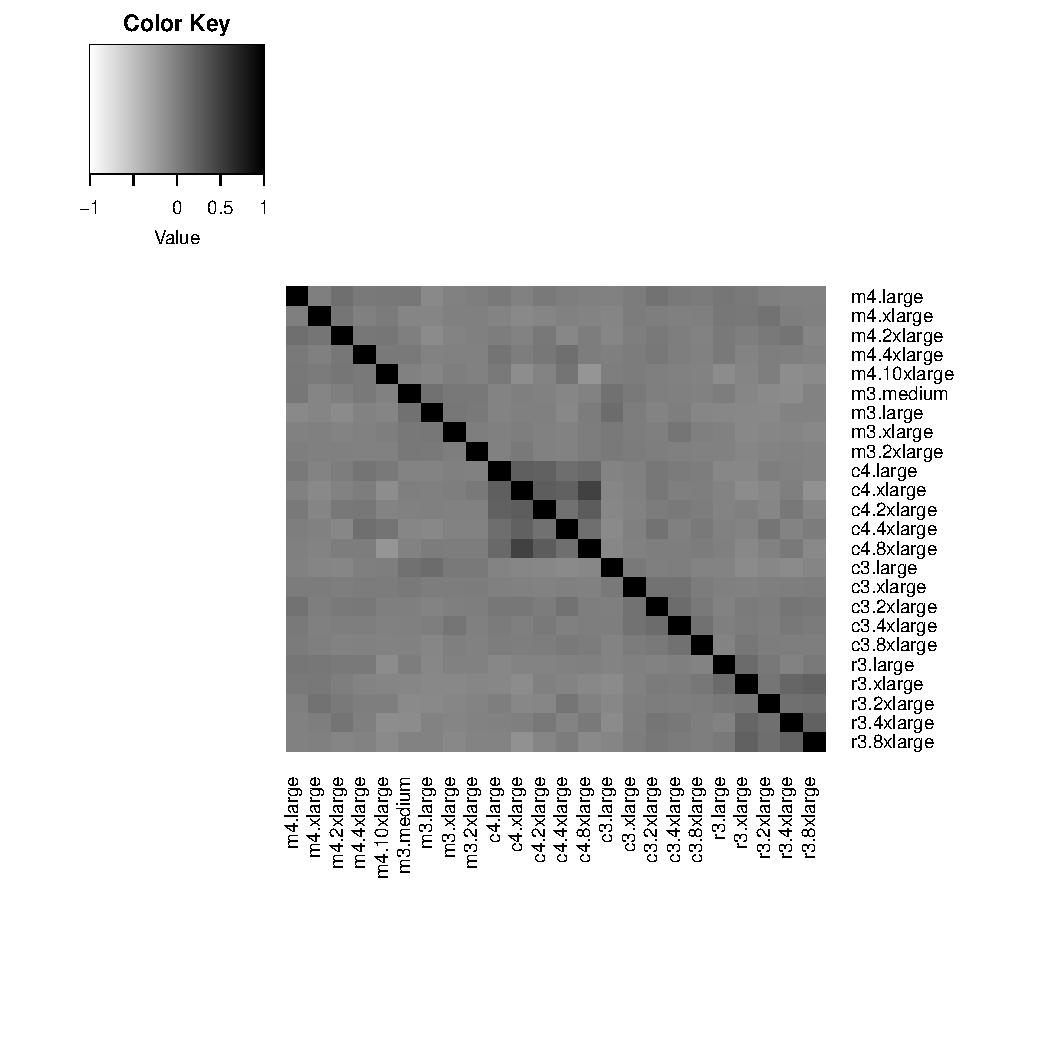
\includegraphics{CorrelationHeatMap}
        \caption{Correlation Between Instance Types}\label{fig:corr}
	\end{center}
\end{figure}

\ref{fig:corr} shows the correlation of each spot instance type with every other spot instance type in the form of a heatmap. As mentioned previously, the closer the value is to zero, the less correlated two server instance types are, and the more negatively correlated they are, the more useful they are for our purposes. In the graph that has been generated, higher positive correlation is shown in darker shades, where black means 100\% positive correlation. Additionally, higher negative correlation is shown in lighter colors, meaning 100\% negative corrleation would be shown in white. This leaves the middle as shades of gray, with the most neutral shades of gray, those closest to the middle between black and white, represent the least total correlation.\par

Before analyzing this data, please note that all data for the t2 instances was empty, as they were too small for the experiments run, and thus their shades should be ignored. Other than this, we can see very clear and very useful trends. The most obvious observation is that the cells representing how correlated an instance is with itself is always black, which should be expected since they are the same data sets. A slightly more subtle trend is that patches of the graph representing "families" of instances, that is to say all instances with the same prefix and thus similar qualities, tend to form patches of the graph that are darker in shade. This is indicative of the fact that there is higher than normal correlation between these families, in general, than there is between instances of two separate families.\par

After these two observations, there is one even more subtle, but potentially more important, that needs to be made. That is that the vast majority of instances are highly uncorrelated. We can see this since the vast majority of squares on this map are a very neutral shade of gray. In looking at the data directly, nearly all correlations are below a factor of +/- 0.1, and nearly all correlations within families are found to be within +/- 0.3. The significance of this is that anything within the +/- 0.3 range is generally considered to be a low "strength of association" \cite{pearsonCoeff}. In other words, excluding a few family member instances, all correlations show very minimal correlation between instance types.\par

Currently, this implication has led to the decision that factoring in correlation when making purchasing decisions is somewhat unnecessary. While it has the potential to provide higher efficiency of choices and may want to be considered later, there are difficulties in using the Pearson Correlation Coefficient that make it not worthy of the effort at the time. The most notable issue is that there is no precise way defined in which to use the coefficient in this way. A correlation of .1 does not represent an exact 10\% positive correlation, the Pearson Correlation merely shows the relative correlation when compared to the correlation coefficient of others. This means that there's no way to know how best to use this factor as an additional consideration after price and availability percentage, and with such little correlation between the vast majority of instance types, it is unnecessary to consider at this time.\par

\section{Cost Comparisons}

\begin{figure}
	\begin{minipage}{0.49\textwidth}
    	\frame{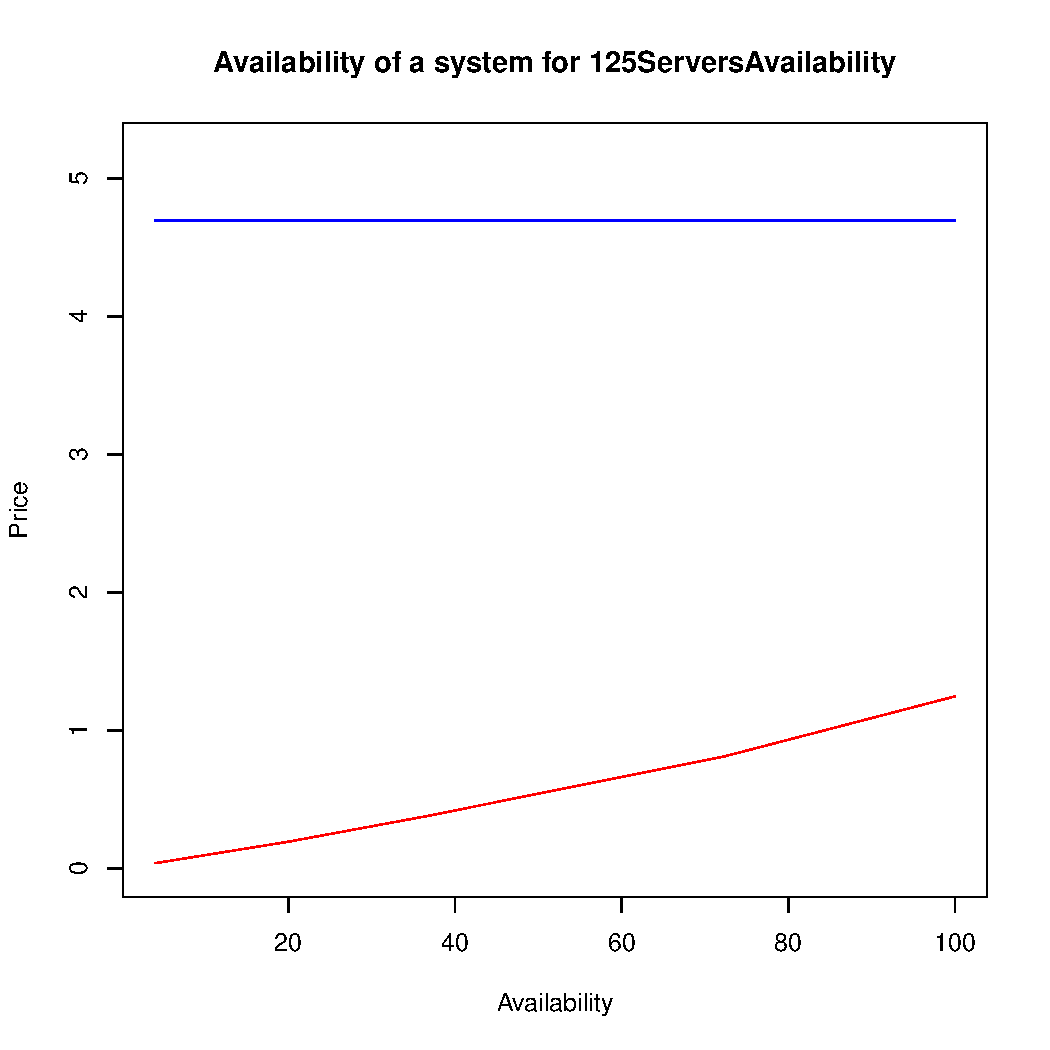
\includegraphics[width=\linewidth]{125ServersAvailability}}
        \caption{125 Servers}\label{Fig:125servercost}
    \end{minipage}
    \begin{minipage}{0.49\textwidth}
    	\frame{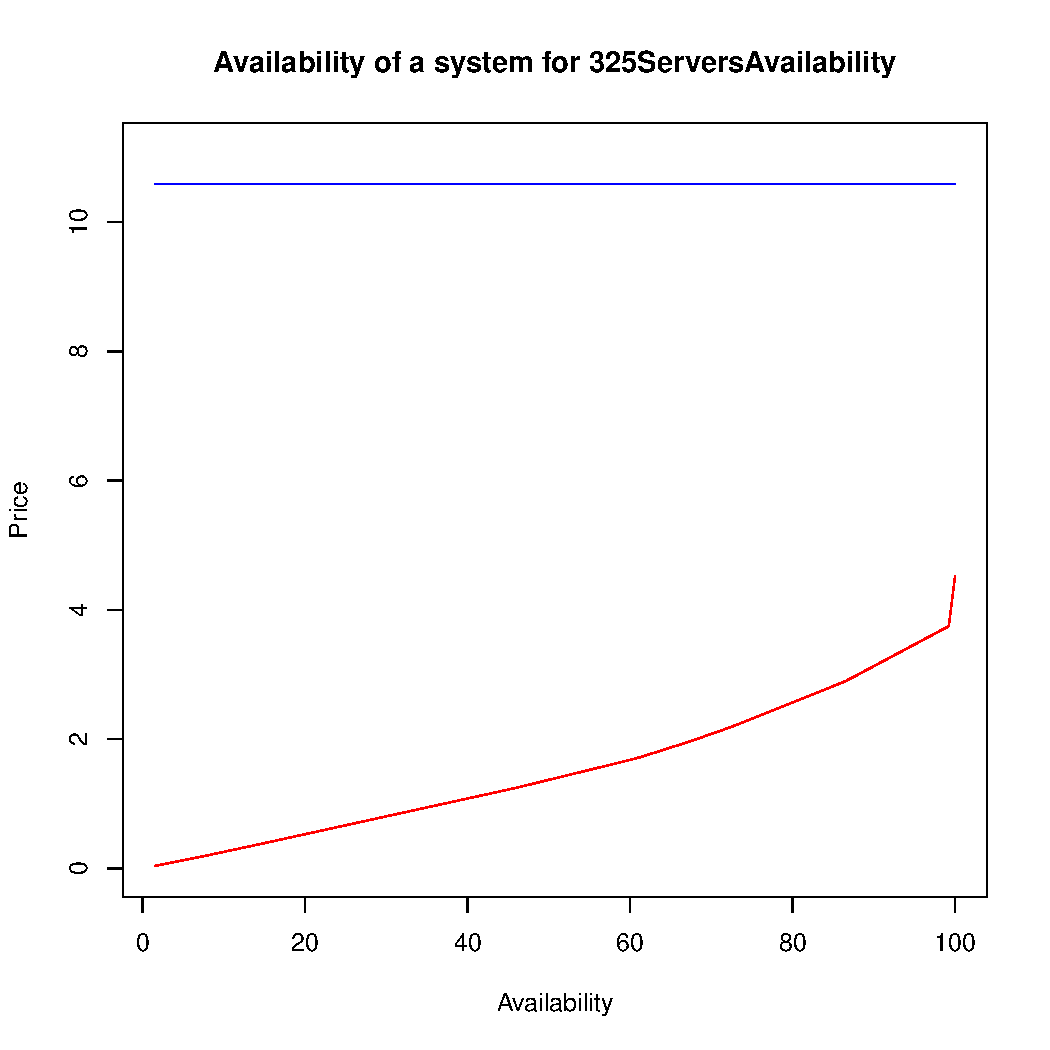
\includegraphics[width=\linewidth]{325ServersAvailability}}
        \caption{325 Servers}\label{Fig:325servercost}
    \end{minipage}
\end{figure}

\ref{Fig:125servercost} and \ref{Fig:325servercost} show our results for a cost analysis at 2 different desired states. In both graphs, the red line represents the cost in terms of dollars per hour to obtain the given availability percentage for BrightSpot. The blue line represents the On-Demand cost for holding that number of baseline server instances. Both graphs show a strikingly similar result, being that the expected cost to utilize BrightSpot for a user's web service is approximately one third of the cost of the On-Demand system implementation. \par

This is clearly a very good sign for moving forward in the BrightSpot implementation. Even if the initial cost calculations have an error of 100\%, we would still end up saving money by utilizing BrightSpot as opposed to an On-Demand implementation of the same system. One might notice that there is a spike at the very end of the BrightSpot cost line in \ref{Fig:325servercost}. This is caused by the greedy algorithm not considering the size of the last obtained resources and, in the case of our testing, it just happened to be the case that the last obtained instance provided many baseline servers. This caused the cost to spike up slightly, however given BrightSpot's secondary use, as well as the slight impact made by this addition, this is not seen as a problematic issue.\par

However, we would have also expected to see a similar spike cost graphs. This is because the higher the availability already is, the less impact an additional server is going to make on total system availability, as it is mostly adding availability that is already covered by other servers. There are two reasons this is not as noticeable in \ref{Fig:125servercost} nor in many other data sets we tested. First, the approximation formula used makes getting an availability accurate to .01\% difficult, so it is likely not ending exactly there and simply gets very close to this value. This is a non-concern in terms of actual system availability, however, because when an instance is lost, BrightSpot will be obtaining replacements immediately, and the extra servers we have already obtained should support the system until then.\par

Another cause for the lack of expected pricing spike would be that in the testing shown, we used a bid that provided above 90\% availability of every instance type, generally above 95\%. This means that just obtaining the correct number of baselines is already nearly reaching our availability goal, so generally the addition of one to two more is all that is needed. When only adding so few, the price continues to increase mostly linearly.


\section{Excess Server Availability}

\begin{figure}
	\begin{minipage}{0.49\textwidth}
    	\frame{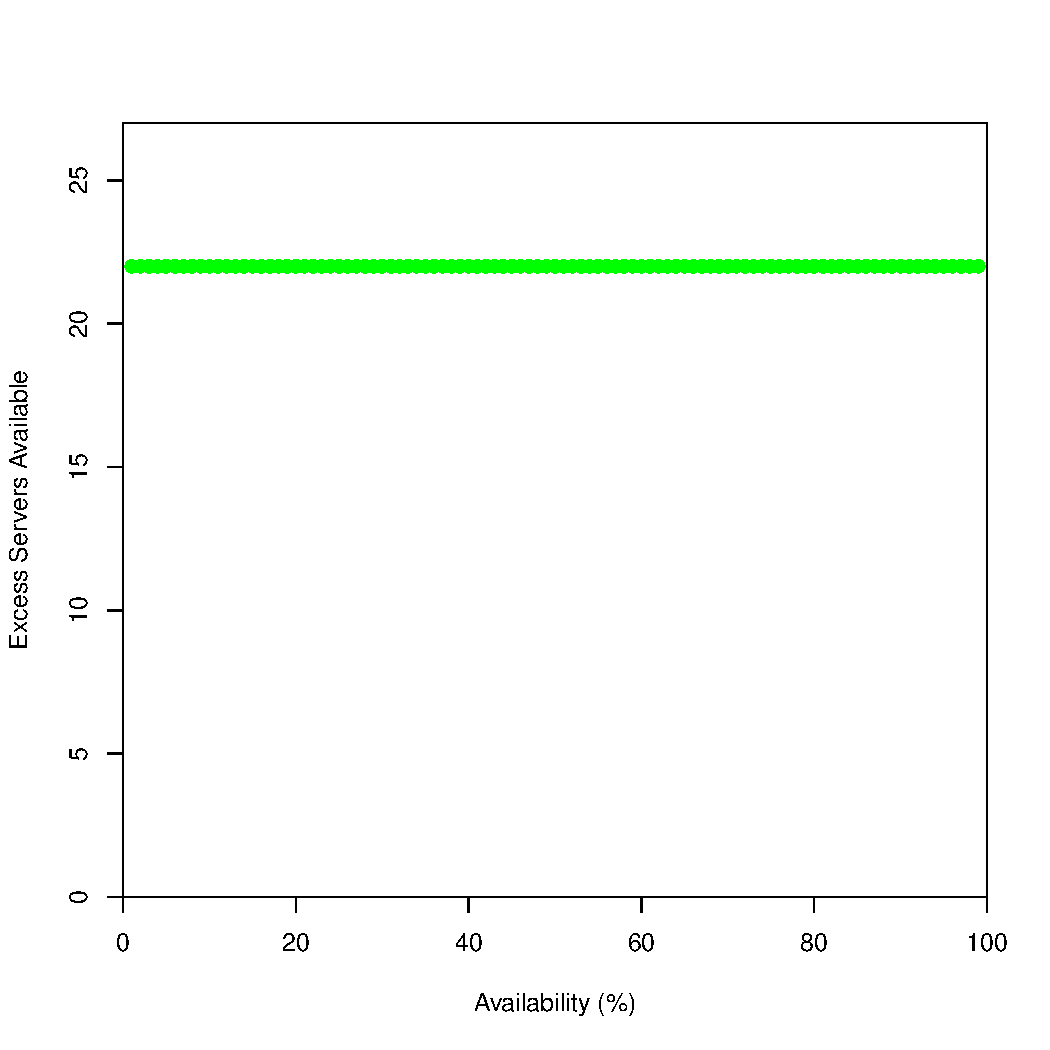
\includegraphics[width=\linewidth]{125ServersAvailabilityExcess}}
        \caption{125 Servers}\label{Fig:125serverexcess}
    \end{minipage}
    \begin{minipage}{0.49\textwidth}
    	\frame{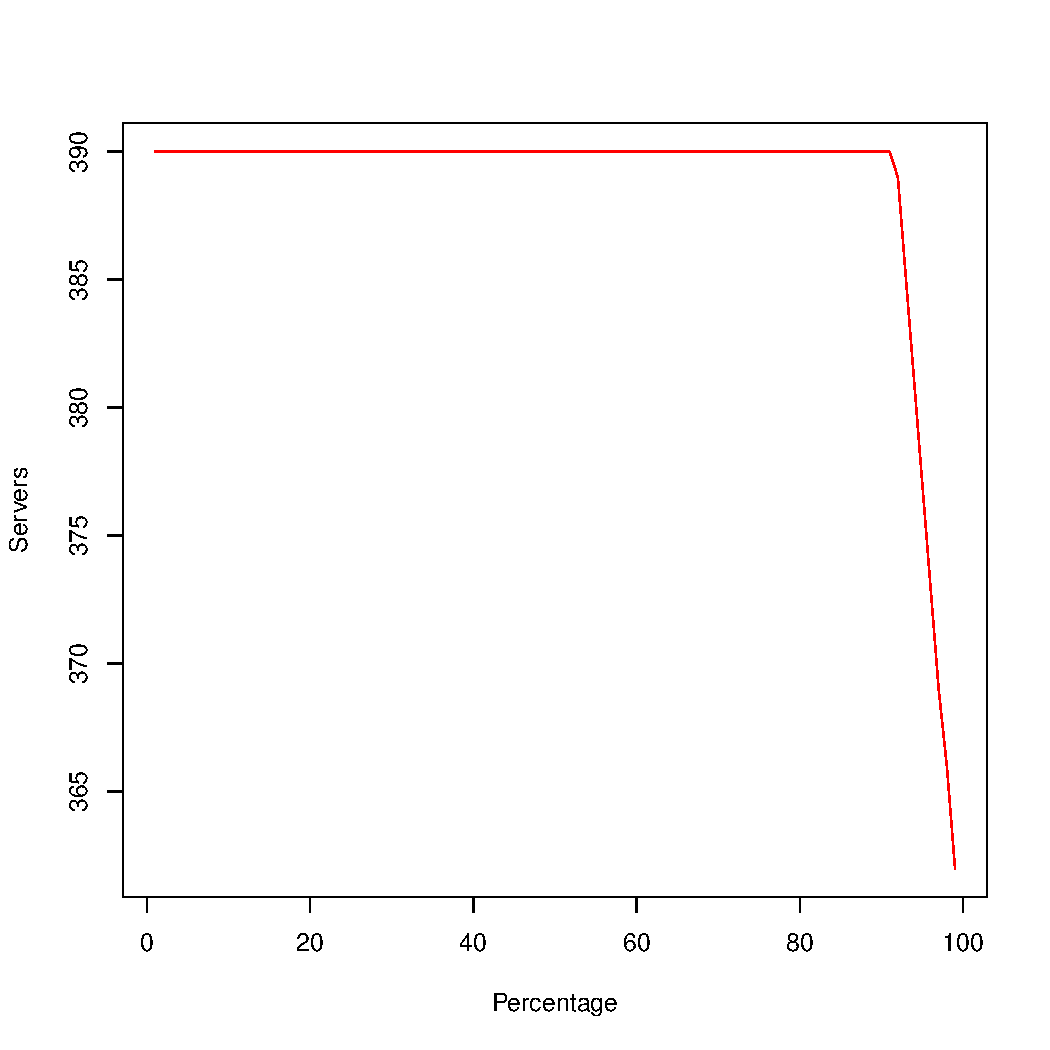
\includegraphics[width=\linewidth]{325ServersAvailabilityExcess}}
        \caption{325 Servers}\label{Fig:325serverexcess}
    \end{minipage}
\end{figure}

Depicted in \ref{Fig:125serverexcess} and \ref{Fig:325serverexcess} one can see the availability of excess servers we have access to. The plot is of the total number of servers available over the percentage of availability. This means that the line depicts the number of total servers available at the percentages displayed on the x-axis. As one can see, thanks to the right bidding strategy producing instances that will be available most of the time to us, generally 90\% of the time or more, the number of total baseline servers available to us is the same as the number of total baseline server instances we have obtained until we aim for very high percentages of availability.\par

If we analyze this data further, we can see exactly how many extra servers we have, multiply that by the percent of the time they are available, choose some length of time, and determine exactly how much excess computing power we have available for us in that time. For instance, if we look at \ref{Fig:325serverexcess}, we see that we have obtained 390 servers for approximately 85\% of the time. Then, we see a fairly steady decline at every percentage until we reach 360 available servers. The loss of 30 baseline servers across 15\% of the time yields a drop of about two servers per percentage point.\par

With this, we can determine how many servers we had at every minute for 100 minutes. For 85 minutes, we have 65 extra servers. For 1 minute, we have 63 extra servers, and so on. Once reasoned out, this yields an average of 62 servers in excess at all times. Using this knowledge, a user may then begin to plan out how to best utilize this space for a background process, such as computationally heavy sorting.




\chapter{Conclusion}

We present BrightSpot, a cost efficient way to implement services on the cloud. The key contribution made by BrightSpot is the ability to create a web service that is available to all users at a desired availability goal for a fraction of the cost of a traditional cloud implementation. Being able to purchase the right spot instances to obtain the highest availability for the minimal cost is pivotal to achieving the best cost to benefit ratio. We have accepted the historical data available from Amazon EC2 to make the best spot instance choices. We now propose to implement BrightSpot on EC2, where it will use Kubernetes to maintain the availability of the system and ensure the availability requested by the user. Once implemented, we will be able to assess how BrightSpot performs compared to the expected cost of operation and to the On-Demand cost of operation. 





%% End of body
%%%%%%%%%%%%%%%%%%%%%%%%%%%%%%%%%%%%%%%%%%%%%%%%%%%%%%%%%%%%%%%%%%%%%%%%%%%%%%%

\appendix
\chapter{THE FIRST APPENDIX TITLE}
...
\chapter{THE SECOND APPENDIX TITLE}
...

%%
%% Beginning of back matter
\backmatter  %% <--- mandatory

%%
%% We don't support endnotes

%%
%% A bibliography is required.
\interlinepenalty=10000  % prevent split bibliography entries
\nocite{*}
\bibliographystyle{umassthesis}
\bibliography{KubernetesThesisBib}

\end{document}

%%% Local Variables: 
%%% mode: latex
%%% TeX-master: t
%%% End: 
